\documentclass[10pt,twocolumn,letterpaper]{article}

\usepackage{cvpr}
\usepackage{times}
\usepackage{epsfig}
\usepackage{graphicx}
\usepackage{amsmath}
\usepackage{amssymb}
\usepackage{gensymb}

\usepackage{stfloats}
\usepackage{tablefootnote}

%%%%%%%% OTHER PACKAGES
\usepackage{float}
\usepackage{caption} % solve for table caption spacing 
\captionsetup[table]{skip=10pt} % to force bib position
\usepackage[section]{placeins}
\usepackage{subcaption}
\usepackage{multirow} % for tabular multi-row
\usepackage{enumitem}
\newcommand{\denselist}{\itemsep -2pt\parsep=1pt\partopsep 0pt}
\newcommand{\bitem}{\begin{itemize}\denselist}
\newcommand{\eitem}{\end{itemize}}
\newcommand{\benum}{\begin{enumerate}\denselist}
\newcommand{\eenum}{\end{enumerate}}
%%%%%%%%%%%%%%%

\usepackage[breaklinks=true,bookmarks=false]{hyperref}

\cvprfinalcopy % *** Uncomment this line for the final submission

\def\cvprPaperID{****} % *** Enter the CVPR Paper ID here
\def\httilde{\mbox{\tt\raisebox{-.5ex}{\symbol{126}}}}

% Pages are numbered in submission mode, and unnumbered in camera-ready
%\ifcvprfinal\pagestyle{empty}\fi
\setcounter{page}{1}
\begin{document}

%%%%%%%%% TITLE
\title{DN Learner: Unsupervised Learning of Depth and Surface Normal from Video}

\author{Aman Raj\\
{\tt\small amraj@eng.ucsd.edu}
% For a paper whose authors are all at the same institution,
% omit the following lines up until the closing ``}''.
% Additional authors and addresses can be added with ``\and'',
% just like the second author.
% To save space, use either the email address or home page, not both
\and
Menghe Zhang\\
{\tt\small mez071@eng.ucsd.edu}
\and
Sarah Wang\\
{\tt\small sawang@eng.ucsd.edu}
\and
Tingwei Yu\\
{\tt\small t3yu@eng.ucsd.edu}}

\maketitle
%\thispagestyle{empty}

%%%%%%%%% ABSTRACT
\begin{abstract}

Learning to reconstruct depths and camera pose from video sequences in an unsupervised approach is attracting significant attention since the work of Zhou et al.\cite{zhou2017unsupervised}. 
%In this work, Zhou proposed an unsupervised framework for monocular depth and camera motion estimation by warping subsequent frames in unstructured video sequences.
Our work extends their work by jointly estimating depth, camera pose and surface normal in an end-to-end framework. We verify that deep learning networks can benefit from explicit geometric cues and constraints provided by instance and semantic-level segmentations. In addition, we enforce the consistency between depth and normal to yield more robust geometrical predictions. Evaluations are performed on the KITTI dataset\cite{kitti} and ablation studies regarding different geometric constraints are also conducted to compare their effectiveness.  

\end{abstract}

%------------------------------------------------------------------------

\section{Introduction}
Inferring camera pose, depth and surface normal of a scene at a detailed level is crucial for 3D scene understanding. The techniques to recover these information from monocular video sequences can be widely applied in various real-world applications. For instance, in robot navigation, this enables the robot to avoid obstacles and travel through unseen areas. Such ability also facilitates 3D reconstruction of the environment and can be applied in the field of augmented reality. 

Recently, there has been large progress in unsupervised pose and depth estimation using monocular cameras. Works such as \cite{zhou2017unsupervised} has significantly reduced human effort to obtain large quantities of ground truth color-depth image pairs for training, while also yielding comparable results to supervised approaches. The key concept is to use view synthesis as supervision by warping a frame in a sequence to the view of its consecutive frames. The work of Yang \textit{et al.}\cite{yang2018lego} refines the estimated depth by leveraging the constraint between surface normal and depth and image gradients to represent edges where depth discontinuities can occur. Casser \textit{et al.}\cite{casser2018depth} takes additional instance-level segmentation along with RGB images as input and predicts poses for the static background and each dynamic object separately. 

In our work, we study the effects of posing different geometric constraints and additional input cues in the form of semantic segmentation to improve geometry predictions. First, we investigate if edge-awareness leads to better depth predictions. Second, we show that by augmenting the input of network with semantic information generates sharper depth results as it provides notion of object boundaries and geometrical consistencies. Lastly, we explore two different methodologies to learn normal. We examine the effect of a weaker depth-normal constraint from \cite{yang2018lego} which forces the normal predictions to be perpendicular to the tangent object plane. Furthermore, we examine patch-based photometric consistency constraint motivated from \cite{furukawa2010accurate} that forces the normal prediction within a patch to be consistent. Evaluation on the KITTI dataset \cite{kitti} demonstrates the effectiveness of different approaches.

%------------------------------------------------------------------------
\section{Related work}
\noindent \textbf{Warping-based view synthesis.}
View synthesis aims to create novel views of a specific subject from images from different view points. Classic paradigm explicitly reconstruct the accurate 3D model of the scene and composite the novel view from the input images \cite{malik1996modeling}\cite{fitzgibbon2005image}\cite{DBLP:journals/tog/ZitnickKUWS04}. An alternative approach is to synthesize images without explicitly estimating the 3D geometry of the scene. For instance, Mahajan \textit{et al.} \cite{shechtman2010regenerative} proposed to move the gradients in the input images along a specific path to reconstruct a novel view. Shechtman \textit{et al.} \cite{shechtman2010regenerative} proposed a patch-based optimization framework to reconstruct new views. The end-to-end learning based framework DeepStereo \cite{DBLP:journals/corr/FlynnNPS15} uses two towers to predict depth and color and fuses them together to reconstruct the scene.  
\\
\noindent
%\textbf{Unsupervised learning of geometry from videos.} 
%Unsupervised learning of visual representations has along history starting from the original auto-encoder work of Olhausen and Field\cite{olshausen1997sparse}. To acquire a compact visual representation, general approaches design pretext tasks to learn visual features, from video data that can later be re-purposed for other vision tasks. Early works such as \cite{zou2012deep} focuses on exploiting geometric constraints in the auto-encoder framework, where they enforce learned representations to be temporally smooth. Similar to this, Goroshin et al.\cite{goroshin2015unsupervised} proposed to learn auto-encoders based on the slowness prior. Other approaches such as Taylor et al.\cite{taylor2010convolutional} trained convolutional gated RBMs to learn latent representations from pairs of subsequent frames. A recent work extended this by learning a LSTM model in an unsupervised manner to predict future frames \cite{srivastava2015unsupervised}.
\\
\textbf{Image segmentation.}
Semantic-level segmentation is a fundamental task in computer vision, where a semantic label is assigned to every pixel. In recent years, deep convolutional neural networks that rely on hand-crafted features showed remarkable improvements on different segmentation benchmark tasks. Among these, the state-of-the-art work DeepLabv3+ \cite{deeplabv3plus2018} uses an atrous spatial pyramid pooling decoder module which refines the segmentation results along object boundaries. In our work, we use DeepLabV3+ model trained on Cityscapes \cite{cordts2016cityscapes} to generate semantics for KITTI. For instance level segmentation we use state-of-the-art Mask-RCNN model \cite{he2017mask} trained on COCO dataset \cite{lin2014microsoft}. We argue that with these additional geometric cues, the network could generate more promising depth predictions with finer details.

%------------------------------------------------------------------------
\section{Method}
The approaches we mention here are used for jointly estimating depths, surface normal and ego-motion. In particular our experiments are focused on improving depth and normal. The core idea is to perform inverse warping from the target view to source view with awareness of the underlying 3D geometry of the scene. 
\subsection{Algorithm Baseline}
The baseline for our algorithms come from Zhou \textit{et al.} \cite{zhou2017unsupervised} having separate models for depth and pose predictions. \\
\noindent \textbf{DepthNet} 
The architecture of DepthNet is taken from \cite{mayer2016dispnet} which uses an encoder followed by a decoder with skip connections and multi-scale side outputs. Other than the final output layer, which has a sigmoid function applied to enforce the predictions in an reasonable range, the other convolution layers are are followed by ReLU activations.\\  
\textbf{PoseNet}
We adopted the PoseNet architecture proposed in \cite{zhou2017unsupervised}. The input of the network is the target-source frame pairs, and the output is the 6D camera pose from each target frame to the source frame. All convolution layers are followed by ReLU activations except for the final output layer, where no non-linear activation is applied. 
%% Here common synthesis
\\
\textbf{View synthesis as supervision} 
Following the notation used in \cite{zhou2017unsupervised}, given a pair of images consisting of a target frame $I_t$ and a source frame $I_s$, we can estimate the depth map $\hat{D_t}$ of the target view and the 6-DOF transformation $\hat{T}_{t\xrightarrow{}s}$ from $I_t$ to $I_s$. Thus, for any pixel $p_t$ in the target frame $I_t$, its corresponding pixel coordinate in the source frame $p_s$ can be found through perspective projection. 

\begin{equation}
    p_s \sim K\hat{T}_{t\xrightarrow{}s}\hat{D_t}(p_t)K^{-1}p_t
\end{equation}

\noindent With this correspondence, a synthesized target view $\hat{I_s}$ can be generated from $I_s$ through bilinear interpolation. By using the target frame as our reference, the photometric loss can be formulated as:

\begin{equation}
    L_{vs} = \sum_s\sum_p |I_t(p) - \hat{I_s}(p)|
\end{equation}
by summing over all pixels $p$ and source images $s$. $\hat{I_s}$ is the source view $I_s$ warped to the target coordinate frame. Now we will explain experiments in subsequent subsections.\\

%% New subsection starts here
\subsection{Edge-aware depth estimation}
In this section, we illustrate two ways to parameterize geometric edges. First we compute the gradient map of target image $I_t$ and synthesized target image $\hat{I_s}$, and require the two gradient images to match as described in \cite{yang2017unsupervised}.
\begin{equation}
    L_g = \sum_{s=1}^S\sum_{x_t}M_s(x_t)||\bigtriangledown I_t(x_t) - \bigtriangledown\hat{I_s}(x_t)||_1
\end{equation}
Here, $M_s(x_t)$ is the explainablitiy mask as in \cite{zhou2017unsupervised}. Since image gradient is robust under lighting condition it consistently encodes the discontinuities in predicted depth. Another way to parameterize edges is to jointly learn the edge map $E_t$ for the target image from semantic mask which is done by directly predicting $E_t$ using a decoder network similar to DepthNet.
\\
\textbf{Regularization of depth} In order to produce smooth depth results, a smooth loss is added for regularization. This loss encourages the estimated depth to be locally similar when no significant image gradient exists, that is 
\begin{equation}
    L_s = \sum_{pt}\sum_{d\in x, y}||\bigtriangledown_d^2D_t(p_t)||e^{-\alpha|\bigtriangledown_dI(p_t)|}
\end{equation}
We use the weight $\lambda_s = 0.5=l$ for this loss term along with common training setup as outlined in Section 4.2.\\
\noindent \textbf{Photometric pixel loss} In addition to the reconstruction loss and smooth loss, Structural Similarity(SSIM)\cite{wang2004image} loss is applied to be part of pixel loss, which is basically window-based pixel comparing, specificly,
\begin{equation}
    L_{pixel} = \alpha_{pixel} \frac{(2\mu_x\mu_y + C_1)(2\sigma_{xy} + C_2)}{(\mu_x^2 + \mu_y^2 + C1)(\sigma_x^2 + \sigma_y^2 + C_2)}
\end{equation}
where $\mu_x$ and $\mu_y$ are averages of $x and y$,while $\sigma_x and \sigma_y$ is the variance.$\sigma_{xy}$ is the covariance. L is the dynamic range of the pixel-values. $c_1=(k_1L)^2$,$c_2=(k_2L)^2$ to stabilize the division with week denominator. We set $k_1=0.01 and k_2=0.03$.
Our best result from these experiments come from using loss terms of Equation 4 and 5 as shown in Table \ref{tab:depth_pred}.

%% New subsection stars here

\subsection{Depth estimation using object motion model with semantic priors}

\begin{figure*}
    \centering
    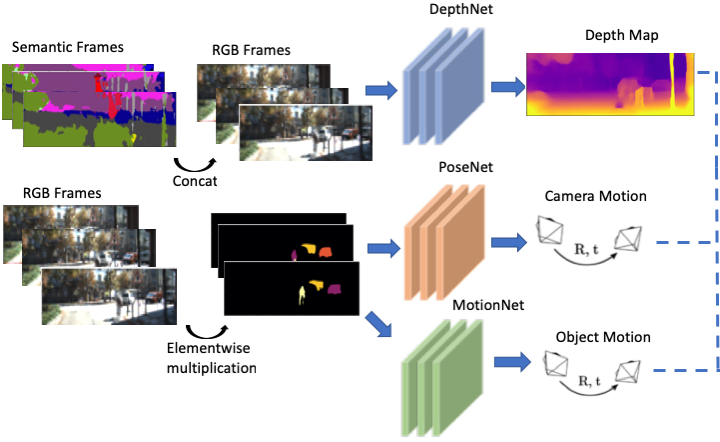
\includegraphics[width=\linewidth, height=6cm]{architecture.png}
    \caption{Our Unsupervised architecture for Subsection 3.3 which contains DepthNet, PoseNet and MotionNet}
    \label{fig:arch}
\end{figure*}

Adapting the work of \cite{casser2018depth} which explicitly models the 3D motion of dynamic objects along with ego-motion of camera, we extend this work further by integrating semantic information of scene to improve depth prediction. Intuitively, semantic information encodes spatial constraints which can explain depth and normal discontinuities. Our DepthNet takes as input RGB sequence along with corresponding semantic segmentation(pixel-wise), encoded in one-hot encoding format. The ego-motion network PoseNet $\phi_{E}$ is used to predict ego-motion of static background and object motion model $\phi_{M}$ is used to predict motion of individual dynamic object. $\phi_{E}$ and $\phi_{M}$ share the same architecture but different inputs. 

We define instance-aligned segmentation masks $(S_{1}, S_{2}, S_{3})$ for corresponding sequence $(I_{1}, I_{2}, I_{3})$. In order to compute ego-motion of static scene only, we define static scene binary mask $(O_{1}, O_{2}, O_{3})$ where $O_{i}$ is binary complement of $S_{i}$. The static binary mask is applied to all images in sequence by element-wise multiplication to mask out dynamic objects before feeding the sequence to ego-motion model:
\begin{multline}
    V = O_{1} \odot O_{2} \odot O_{3} 
    \\
 E_{1\rightarrow2}, E_{2\rightarrow3} = \phi_{E}(I_{1} \odot V, I_{2} \odot V, I_{3} \odot V) 
\end{multline}

\noindent To compute object motion model, we first apply ego-motion estimates to get warped RGB sequences $(\hat I_{1\rightarrow2}, I_{2}, \hat I_{3\rightarrow2})$ and instance-aligned segmentation sequences $(\hat S_{1\rightarrow2}, S_{2}, \hat S_{3\rightarrow2})$. Now, for every object instance in image, the object motion estimate $M^{(i)}$ of the \textit{i}-th object is computed as:
\begin{multline}
        M_{1\rightarrow2}^{(i)}, M_{2\rightarrow3}^{(i)} = \phi_{M}(\hat I_{1\rightarrow2} \odot \psi_{i}(\hat S_{1\rightarrow2}),
    \\
    I_{2} \odot \psi_{i}(S_{2}), \hat I_{3\rightarrow2} \odot \psi_{i}(\hat S_{3\rightarrow2})
\end{multline}

\noindent where $M_{1\rightarrow2}^{(i)}, M_{1\rightarrow2}^{(i)} \in \mathbb{R}^{6}$ and $\psi_{i}(S_{1})$ returns binary mask only for object \textit{i} in  $S_{1}$. Now, corresponding to these motion estimates, inverse warping is done to move the objects according to predicted motions. This is done by first warping the full image using motion estimate and then masking out the corresponding object. For example, $\hat I_{1\rightarrow2}^{(i)}$ is obtained by using motion estimate $M_{1\rightarrow2}^{(i)}$. Final warped image  $\hat I_{1\rightarrow2}^{(F)}$ is a combination of warped static background and individual warping of each dynamic object given by:

\begin{multline}
\hat I_{1\rightarrow2}^{(F)} = \hat I_{1\rightarrow2} \odot V + \sum_{i=1}^{N} \hat I_{1\rightarrow2}^{(i)} \odot \psi_{i}(S_{2})
\end{multline}

\noindent Equivalent for $\hat I_{3\rightarrow2}^{(F)}$ can be found using above Equation 8. We also impose object size constraint as in \cite{casser2018depth}, to make sure the network is learning reasonable depth matching object motion estimates. The architecture overview of this method can be found in Figure \ref{fig:arch}. We obtained our best depth prediction result using this approach which is mentioned in Table \ref{tab:depth_pred}. We also show some qualitative results of this method in Figure \ref{fig:depth_result}.

%% New subsection starts here
\subsection{Depth-normal consistency constraints}
For surface normal estimation, we build NormalNet by modifying the architecture of DepthNet such that it shares the same encoder of DepthNet while having a separate decoder to predict surface normal. While training, we jointly train the decoder branches of both the networks. 
\subsubsection{Depth and normal orthogonality constraint.}
To train NormalNet, we applied the depth-normal orthogonality constraint proposed in \cite{yang2017unsupervised} to our network. This could enforce the predicted surface normal to be perpendicular to its tangent plane. For each pixel $x_i$ in the target view, we compute sum of the absolute dot products between the estimated normal and the vectors pointing from the pixel to it's 8 neighbors as shown in Figure \ref{fig:8point}. The loss term can be given by:

\begin{multline}
     L_{orth} = \sum_{i\in t}\sum_{j\in Nei(i)}||[ \phi(x_j) - \phi(x_i)] \hat{N_t}(x_i)||_1 \\ 
    where\ \phi(x) = D_t(x)K^{-1}x 
\end{multline}

\noindent where $Nei(x_i)$ denotes the set of 8 neighboring pixels of $x_i$, $K$ the camera intrinsic matrix and $\hat N(x_i)$ and $\hat D(x_i)$ the estimated surface normal and depth of the corresponding pixel, respectively. We define $\phi(x_i)$ as the back-projected 3D point of pixel $x_i$ in the 3D space, thus $\phi(x_j) - \phi(x_i)$ is the vector pointing from the center pixel to the neighboring pixels in the world coordinates. Since we don't have direct supervision for surface normal, training with $L_{orth}$ would result into the network always predicting zero for the elements in $\hat{N}$. Therefore, an extra regularization term is added in the the loss function to encourage the predicted surface normal to have a unit length. Our best result using this method comes with semantic as additional input. We show the results of the same in Table \ref{tab:depth_pred}. Some qualitative result of this method is shown in Figure \ref{normal:depth}a.

\subsubsection{Patch-based depth and normal constraint.} 
Through experiments we observed that by only enforcing the depth and normal orthogonality correlation could not provide our network enough geometry cues to reconstruct the surface normal(Figure \ref{normal:depth}a). Thus, we applied the patched-based depth and normal constraint to our network based on previous work of \cite{furukawa2010accurate}. For each pixel in the target image, we reconstructed a $\mu \times \mu$ patch $p$ in the 3D space with the center calculated by back-projecting the pixel (Figure  \ref{fig:patch}). The orientation of the patch is given by the estimated surface normal and we assign one of its edges to be parallel to the \textit{x}-axis of the target frame. Through re-projecting each patch back in to the target image $I_t$ as well as the source image $I_s$, we sample the intensities of the patch in both views through bilinear interpolation to acquire $I_{t,p_i}$ and $I_{s,p_i}$. The loss term $L_{patch}$ is then the sum of \textit{L1} difference of the intensities between each pair of patches. Some qualitative result of this method is shown in Figure \ref{normal:depth}b.
\begin{figure}
  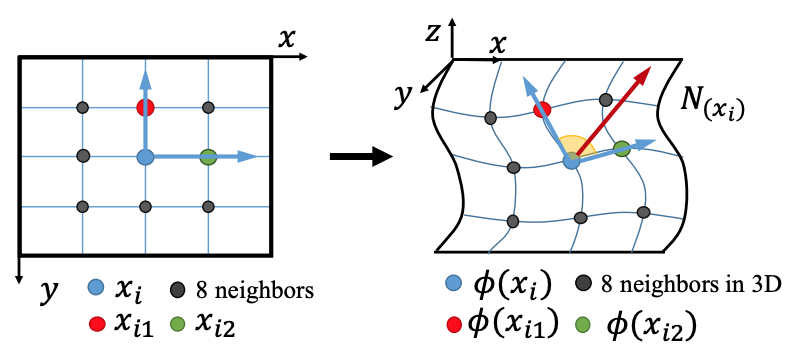
\includegraphics[width=\columnwidth ]{8point.png}
  \caption{Depth and normal orthogonality constraint. To enforce the predicted surface to be perpendicular to the tangent surface, we compute the dot product between the estimated normal and the 8 vectors pointing from the center pixel to the neighboring pixels.}
  \label{fig:8point}
\end{figure}
\begin{figure}
  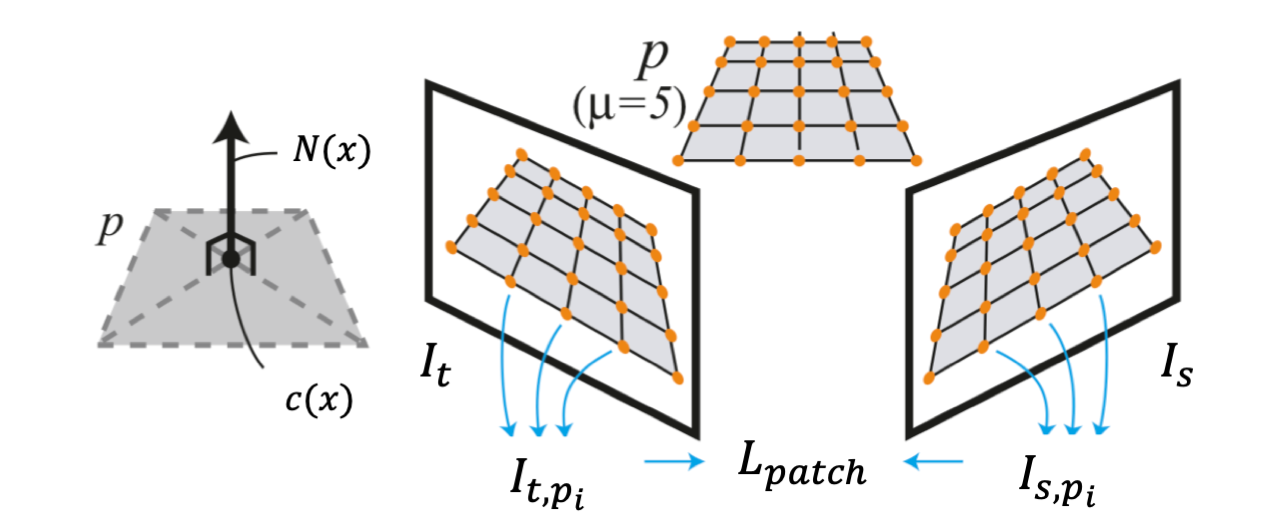
\includegraphics[width=\columnwidth ]{patch.png}
  \caption{Patched-based depth and normal constraint. For each pixel, we reconstruct a patch in the 3D space. The center of the patch $c(x)$ is obtained by back-projecting the pixel with the estimated depth, intrinsic matrix and extrinsic matrix. The orientation of the patch is given by estimated normal $N(x)$.}
  \label{fig:patch}
\end{figure}
\begin{figure}
  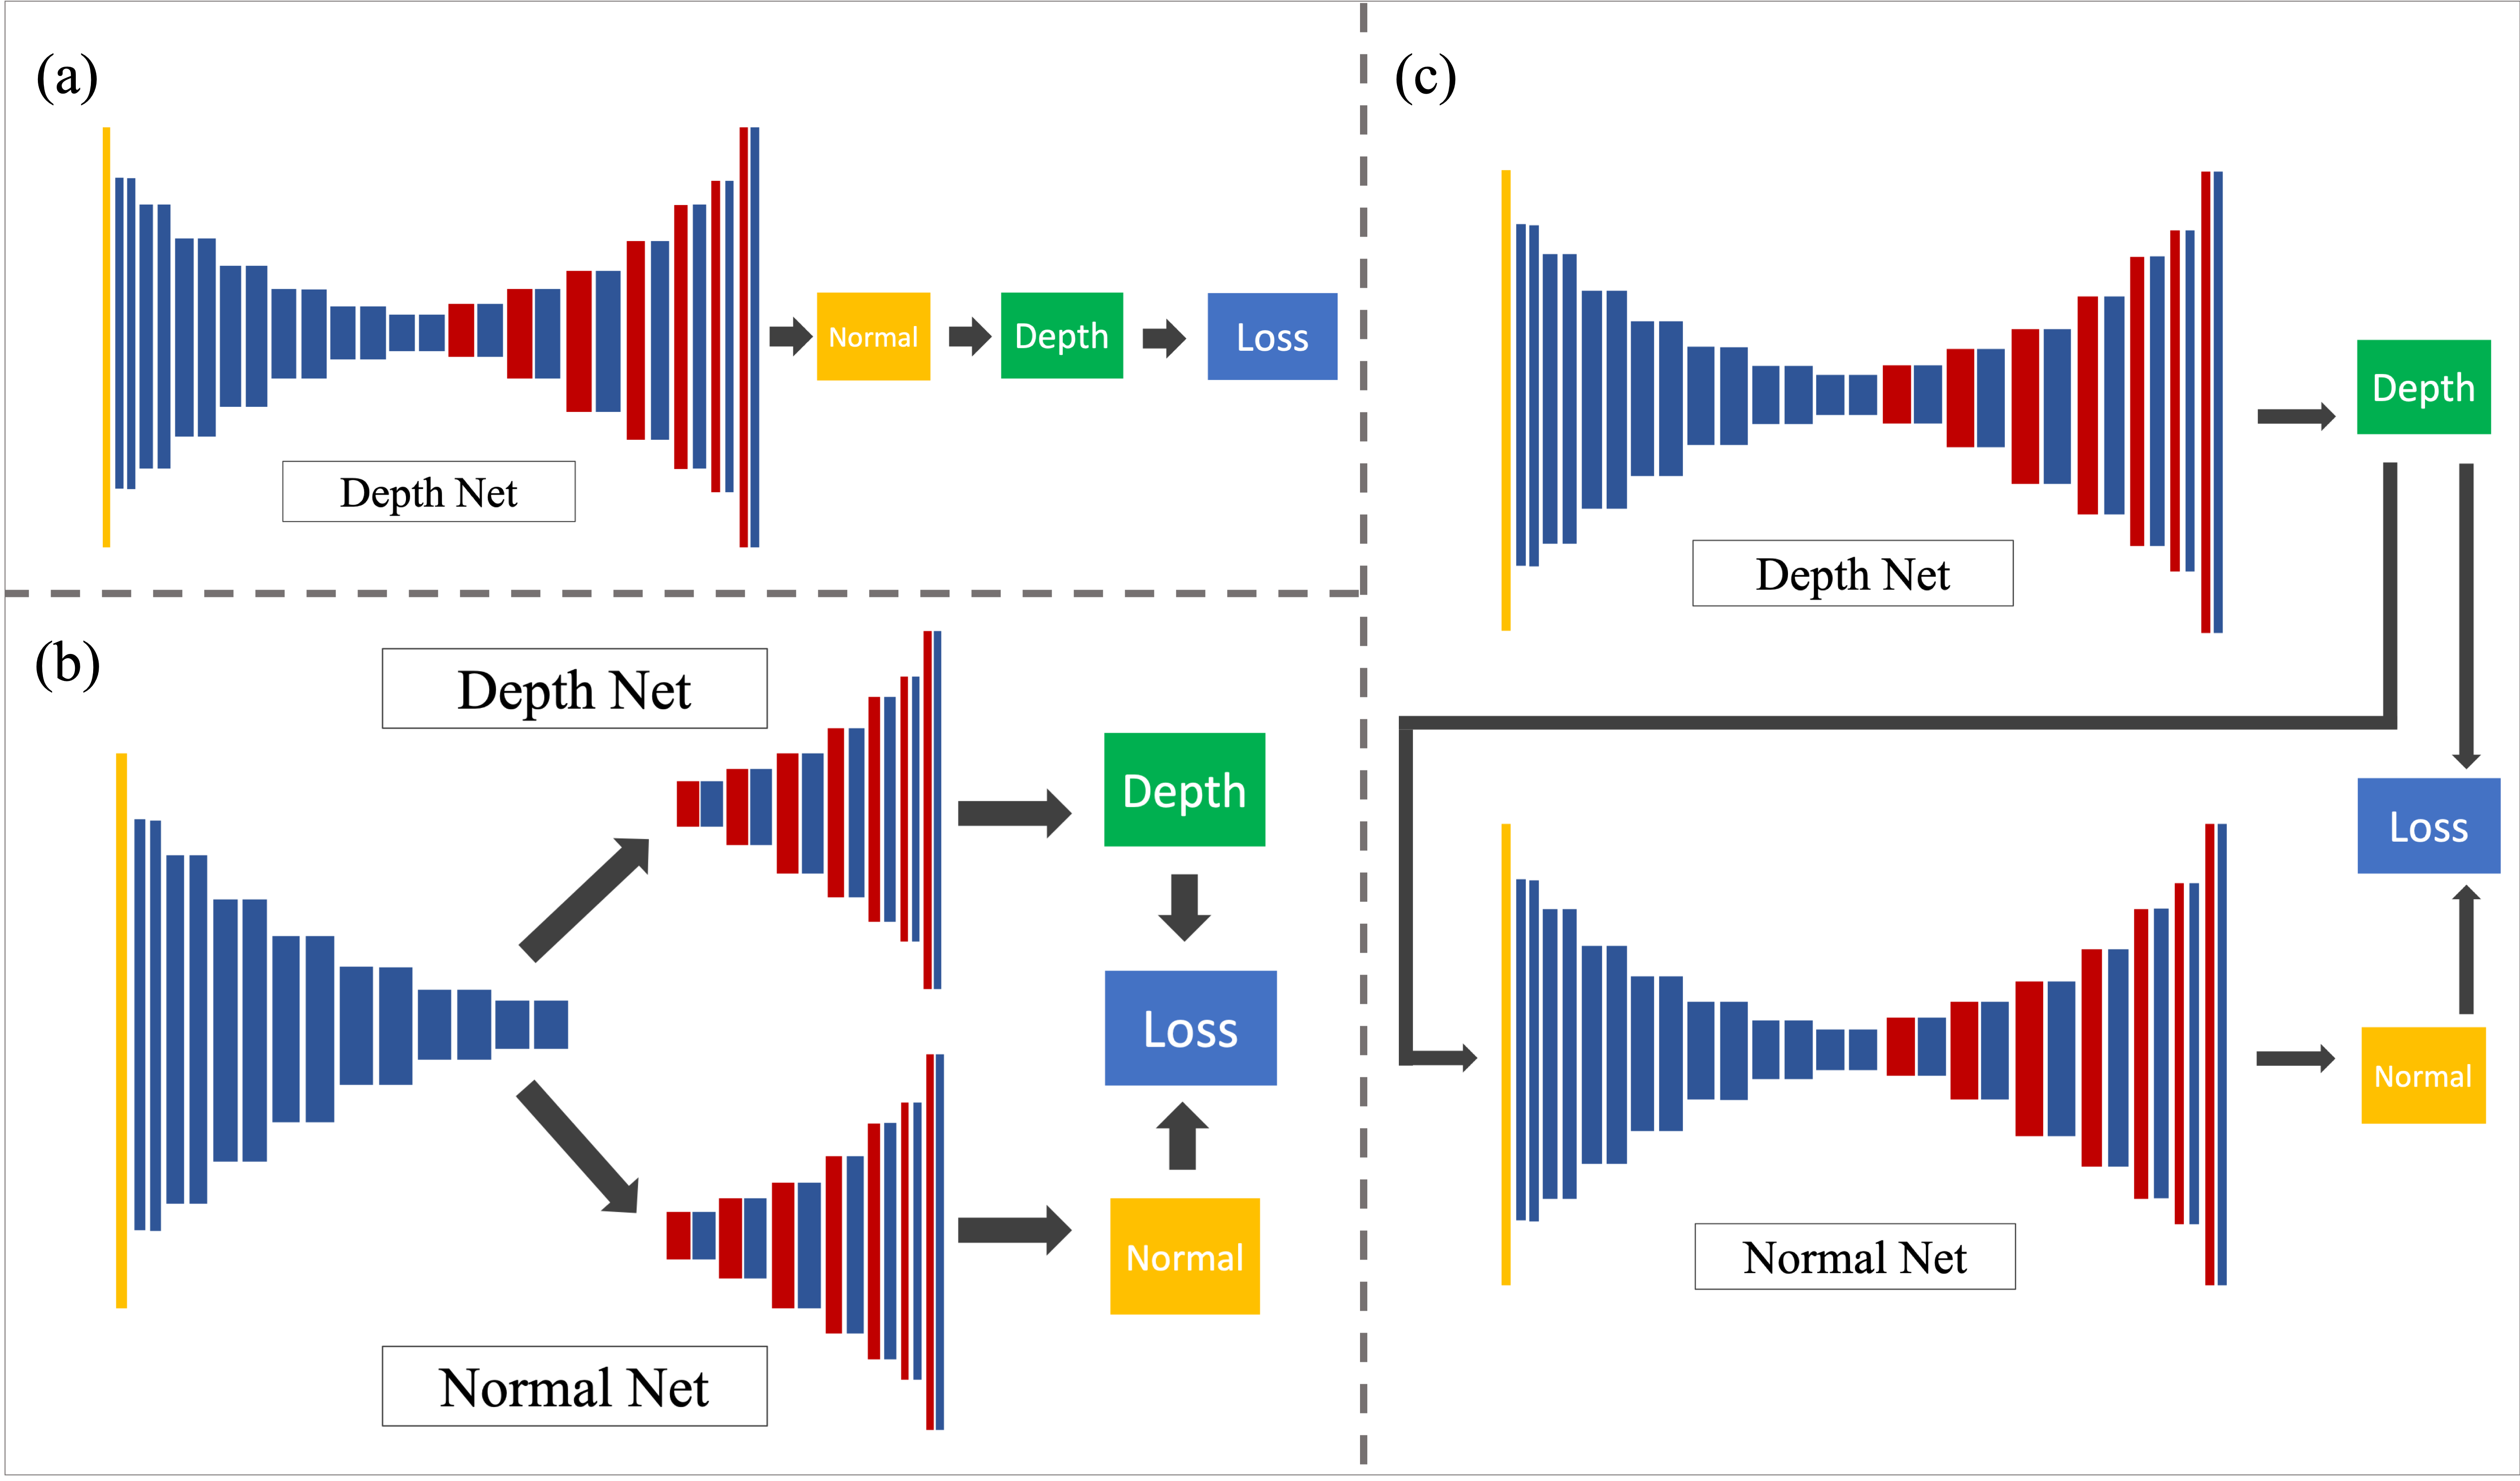
\includegraphics[width=\columnwidth ]{network.png}
  \caption{Network architectures for different experiments. (a) For the edge-aware experiments, the network architecture is based on (include related work), where we compute the normal directly from the predicted depth. (b)While evaluating the patch based photo-consistency constraints, the normal and depth net shares a single encoder and uses different decoders to separately predict depth. (c)To train the normal network with only the depth and normal orthogonality constraint, we froze the depth network and individually trained the normal network with an additional estimated depth input to get reasonable results.}
  \label{fig:network}
\end{figure}

\begin{figure*}[ht]
  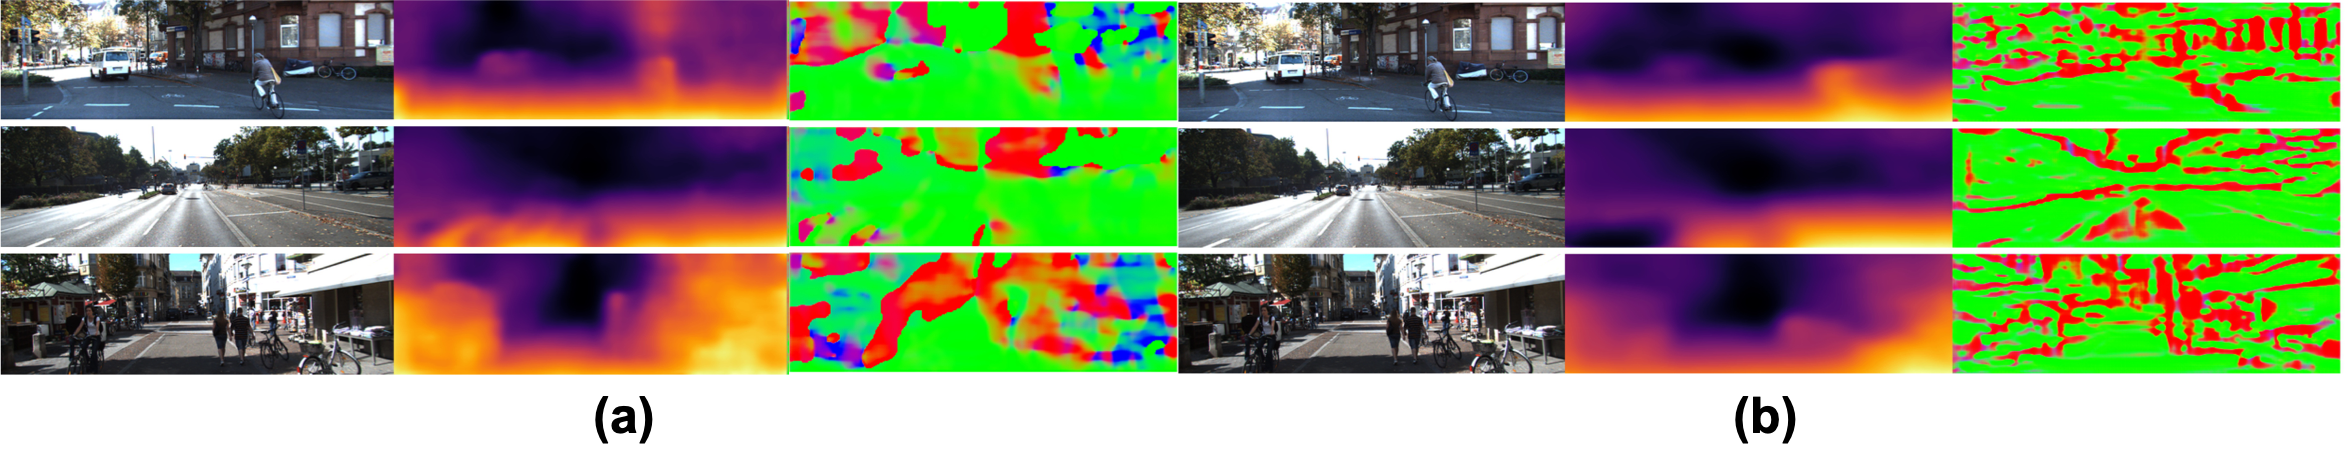
\includegraphics[width=\linewidth]{depth_KITTI.png}
  \caption{(a) Experiment results on KITTI with only the depth and normal constraint mentioned in Subsection 3.4.1 (b) Patch-based experiment results on KITTI mentioned in Subsection 3.4.2}
\label{normal:depth}
\end{figure*}

%% Depth Result Tabl Here
\begin{table*}[htbp]
\centering
\begin{tabular}{ c||c| c c c c|c c c  }
 \hline
  \multirow{2}{*}{Method} & \multirow{2}{*}{Supervised} & \multicolumn{4}{c|}{Error-related metrics} & \multicolumn{3}{c}{Accuracy-related metrics}\\
  &   & Abs Rel & Sq Rel & RSME & RSME log & $\delta < 1.25$ & $\delta < 1.25^2$ & $\delta < 1.25^3$\\
 \hline
 
  Eigen \textit{et al.} \cite{eigen2014depth} Fine & Depth & 0.203 & 1.548 & 6.307 & 0.282 & 0.702 & 0.890 & 0.957 \\

  Liu \textit{et al.}  \cite{liu2016learning} & Depth & 0.202 & 1.614 & 6.523 & 0.275 & 0.678 & 0.895 & 0.965 \\

  Zhou \textit{et al.} \cite{zhou2017unsupervised}(updated) & No & 0.183 & 1.595 & 6.709 & 0.270 & 0.734 & 0.902 & 0.959\\
  
  Yang \textit{et al.} \cite{yang2018lego} & No & 0.162 & 1.352 & 6.276 & 0.252 & 0.783 & 0.921 & 0.969\\

  Yin \textit{et al.} \cite{yin2018geonet} & No & 0.155 & 1.296 & 5.857 & 0.233 & 0.793 & 0.931 & 0.973 \\
  
  Casser \textit{et al.} \cite{casser2018depth}(C) & No & 0.146 & 1.147 & 5.386 & 0.218 & 0.810 & 0.942 & 0.978 \\
 
  Casser \textit{et al.} \cite{casser2018depth}(R) & No & \textbf{0.108} & \textbf{0.825} & \textbf{4.750} & \textbf{0.186} & \textbf{0.873} & \textbf{0.957} & \textbf{0.982} \\

  \hline

  Ours(sub section 3.4.1) & No & 0.173 & 2.095
 & 6.297 & 0.257 & 0.777 & 0.923 & 0.923 \\
  % gradient method edge-aware+SSIM
  Ours(sub section 3.2) & No &  0.206 & 2.860 & 6.969 & 0.278 & 0.734 & 0.901 &     0.956 \\
  
  \textbf{Ours(sub section 3.3)} & No & \textbf{0.140} &     \textbf{1.059} &     \textbf{5.374} &     \textbf{0.215} &     \textbf{0.816} &     \textbf{0.942} &     \textbf{0.978}\\
 \hline
\end{tabular}
\caption{Monocular depth results on the KITTI 2015 \cite{kitti} by the split of Eigen \textit{et al.} \cite{eigen2014depth}. Result of Casser \textit{et al.} (C) is obtained using their provided checkpoint. Casser \textit{et al.} (R) is taken from their paper that has additional refinement during test time. Ours(Subsection 3.3) based on work of \cite{casser2018depth} doesn't use refinement but beats result of provided checkpoint.} \label{tab:depth_pred}
\end{table*}

\section{Experiments}

\subsection{Datasets and metrics}
We conduct experiments on depth and normal estimation. The performances are evaluated on the KITTI dataset \cite{kitti}. For depth evaluation, we adopt metrics used in Zhou \textit{et al.} \cite{zhou2017unsupervised}, details are shown in Table \ref{table1:depth_eval}.

%%%%%%%%%%%%%%% RESULT
\begin{figure}[t]
  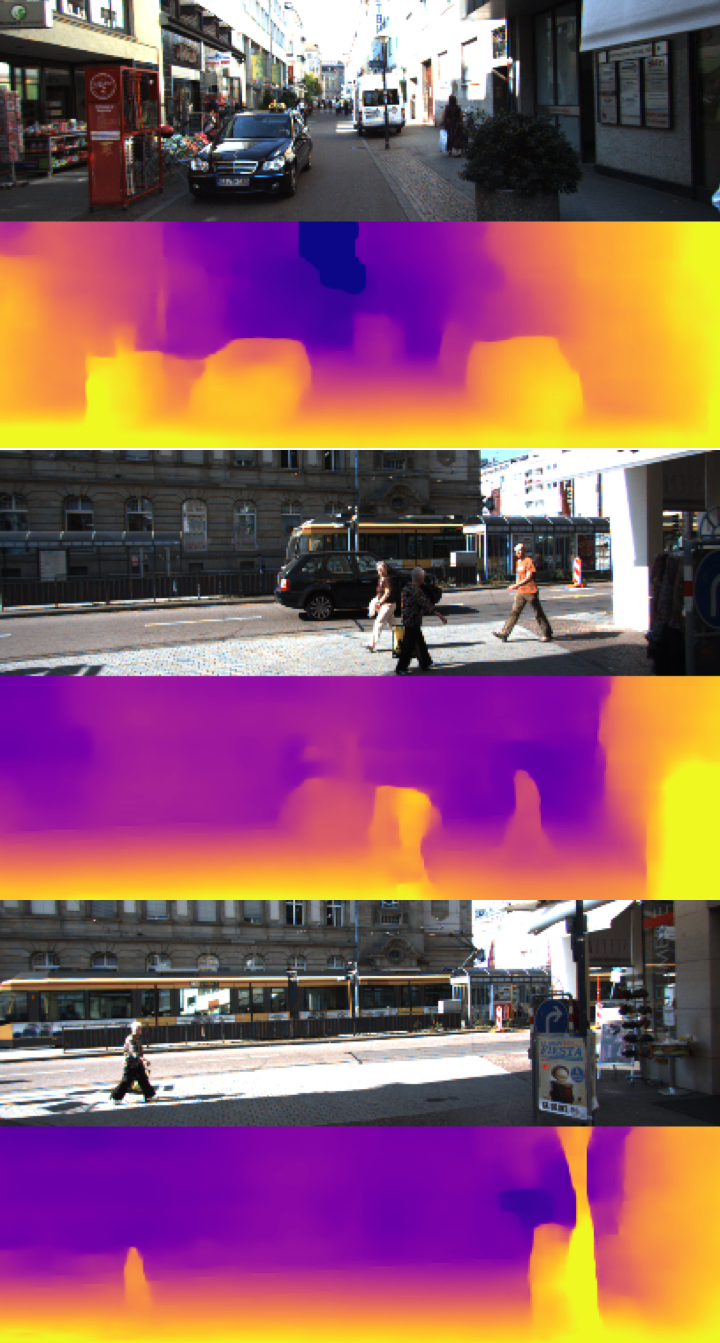
\includegraphics[width=\columnwidth]{dresult.png}
  \caption{Depth-result using our overall best model using the method from Subsection 3.3.}
  \label{fig:depth_result}
\end{figure}

\subsection{Training}

\begin{table*}
\centering
\begin{tabular}{l|l}
 Threshold: $\% of y_i, s.t. max(\frac{y_i}{y_i^*}, \frac{y_i^*}{y_i})=\delta < thr $&  RMSE(linear):$\sqrt{\frac{1}{|T|}\sum_{y\inT}||y_i - y_i^*||^2}$ \\
 Abs Relative difference: $\frac{1}{|T|}\sum_{y\in T||y-y^*||/y^*}$ &  RMSE(log):$\sqrt{\frac{1}{|T|}\sum_{y \in T}||log y_i - log y_i^*||^2}$ \\
 Squared Relative difference:$\frac{1}{|T|}\sum_{y\in T||y-y^*||^2/y^*}$ & 
\end{tabular}
\caption{Depth evaluation metrics}\label{table1:depth_eval}
\end{table*}

Similar to \cite{zhou2017unsupervised}, we implemented the system using TensorFlow framework along with photo-consistency loss $L_{vs}$. For all the experiments, the common setup is: Adam optimizer with $\beta_1 = 0.9$, $\beta_2 = 0.999$, learning rate of $0.0002$ and mini-batch size of 4. All the experiments are performed with image sequences of size 3. We resize the images to $128 \times 416$ during training. We use the eigen split of KITTI for training and evaluation. Additional experimental setups for different methods are outlined below.

%Similar to \cite{zhou2017unsupervised}, we implemented the system using TensorFlow framework. For all the experiments, we set $\lambda_s = 0.5=l$ (l is the downs-caling factor for the corresponding scale) and $\lambda_e = 0.2$. During training, we used batch normalization for all the layers except for the output layers, and the Adam optimizer with $\beta_1 = 0.9$, $\beta_2 = 0.999$, learning rate of $0.0002$ and mini-batch size of 4. The training typically converges after about 150K iterations. All the experiments are performed with image sequences captured with a monocular camera. We resize the images to $128 × 416$ during training.
%Similar to Yang et al.\cite{yang2018lego}, we evaluate the normal map(either from direct-prediction or from depth inference) by comparing to the ground truth normal, which is generated by applying depth-to-normal layer on interpolated depth ground truth. The normal evaluation is performed
%on KITTI dataset. The comparison of normal evaluations on KITTI split is presented in???. \\

\noindent \textbf{Edge-aware depth experiments.}
Architecture for approach outlined in Subsection 3.2 is shown in Figure \ref{fig:network}a. We obtain the surface normal computed using the estimated depth and calculate the loss as mentioned in \cite{yang2017unsupervised}. The best result that we got was with regularization loss $L_s$ set to 0.5 and $L_{pixel}$ set to 0.3 with RGB as input. The result of same is shown in Table \ref{tab:depth_pred}.
%when the input is the RGB image only. When using the semantic mask as an additional input to the network, we set the edge-weight to 0.3.
%To leverage the predicted surface normal in our loss function, we also added smooth loss term for surface normal as we did for the depth and the weight is set to 0.5. The results are shown in the \ref{table1:depth_eval}.

\noindent \textbf{Evaluation on the depth and normal orthogonality constraint.}
We set the weight of $L_{orth}$ to 0.001. Yet, the results aren't very promising as can be seen in Table \ref{tab:depth_pred}. The network can not generate meaningful surface normal and also impaired the depth predictions. Thus, we independently train the NormalNet along with the pre-trained DepthNet to obtain more meaningful results shown in Figure \ref{fig:network}c. As can be seen in Figure \ref{normal:depth}, we can roughly determine the road of the scene but geometric details are coarse.

\noindent \textbf{Evaluation on the patch-based photometric constraint.}
We evaluate the patch-based photometric constraint by adding the $L_{patch}$ term in our loss function and setting its weight to 0.1. We implement the network architecture of this experiment as shown in Figure \ref{fig:network}b. In Figure \ref{normal:depth} we show a qualitative result of this approach. As can been seen, the estimated normal could roughly capture the contours of the scene; however, there are still some spurious blobs in the image. 

%------------------------------------------------------------------------
\section{Conclusion and Future Work}

We tried several approaches to estimate better depth and normal predictions by offering geometric cues and constraints. In our experiments, we observed that both instance-level and semantic information generate more desirable depth results. Our best depth estimation approach uses instance-level segmentation to model dynamic object motion along with semantic priors(Subsection 3.3). Also, we observed that by restraining the network with the depth and normal orthogonality and patch-based constraint, we can also estimate the surface normal of the scene, which is beneficial for future applications. 

In the future, we plan to experiment the refinement methodology as explained in \cite{casser2018depth} to further improve the depth prediction of our best approach. Currently, since our NormalNet is incapable of generating high quality normal maps as compared to non-learning based approaches, we will continue to improve our network with different geometric constraints and architectural designs. Lastly, we would like to show scalability of our approach on different dataset like Cityscape and Make3D.

%------------------------------------------------------------------------

% \begin{table}
% \begin{center}
% \begin{tabular}{|l|c|}
% \hline
% Method & Frobnability \\
% \hline\hline
% Theirs & Frumpy \\
% Yours & Frobbly \\
% Ours & Makes one's heart Frob\\
% \hline
% \end{tabular}
% \end{center}
% \caption{Results.   Ours is better.}
% \end{table}

% {\small\begin{verbatim}
%   \usepackage[dvips]{graphicx} ...
%   \includegraphics[width=0.8\linewidth]
%                   {myfile.eps}
% \end{verbatim}
% }
% \begin{figure}[t]
% \begin{center}
% \fbox{\rule{0pt}{2in} \rule{0.9\linewidth}{0pt}}
%   %\includegraphics[width=0.8\linewidth]{egfigure.eps}
% \end{center}
%   \caption{Example of caption.  It is set in Roman so that mathematics
%   (always set in Roman: $B \sin A = A \sin B$) may be included without an
%   ugly clash.}
% \label{fig:long}
% \label{fig:onecol}
% \end{figure}



% \begin{figure*}
% \begin{center}
% \fbox{\rule{0pt}{2in} \rule{.9\linewidth}{0pt}}
% \end{center}
%   \caption{Example of a short caption, which should be centered.}
% \label{fig:short}
% \end{figure*}



{\small
\bibliographystyle{ieee}
\bibliography{refs}
}

\end{document}
